\documentclass[amsmath, amssymb, aip, jmp, reprint]{revtex4-2}
\usepackage{tikz}
\usetikzlibrary{shapes.geometric}
\usetikzlibrary{decorations.markings}

\begin{document}

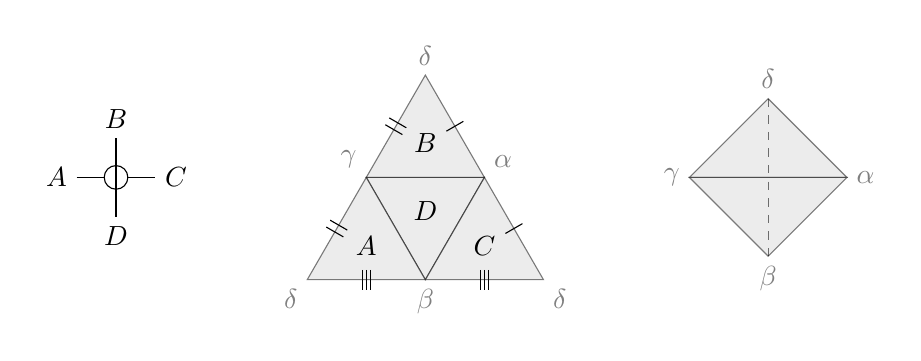
\begin{tikzpicture}
\matrix[column sep = 1 cm]{

	% Graph representation of vertex

	\draw (2.5, 0) node [left] {$A$} -- (3.5, 0) node [right] {$C$};
	\draw [fill = white] (3, 0) circle (0.15);
	\draw (3, -0.5) node [below] {$D$} -- (3, 0.5) node [above] {$B$};

&

	\begin{scope}[yshift = -0.433 cm]		% Shift downward by sqrt(3) / 4

		% Triangles w/ corner labels
	
		\draw [fill = gray!30, semitransparent] (30 : {sqrt(3) / 2}) node [above right] {$\alpha$} -- (150 : {sqrt(3) / 2}) node [above left] {$\gamma$}
			-- (270 : {sqrt(3) / 2}) node [below] {$\beta$} -- cycle;
		\draw [fill = gray!30, semitransparent] (210 : {sqrt(3)}) node [below left] {$\delta$} -- (150 : {sqrt(3) / 2}) -- (270 : {sqrt(3) / 2}) -- cycle;
		\draw [fill = gray!30, semitransparent] (30 : {sqrt(3) / 2}) -- (270 : {sqrt(3) / 2}) -- (330 : {sqrt(3)}) node [below right] {$\delta$} -- cycle;
		\draw [fill = gray!30, semitransparent] (30 : {sqrt(3) / 2}) -- (150 : {sqrt(3) / 2}) -- (90 : {sqrt(3)}) node [above] {$\delta$} -- cycle;
	
		% Face labels
	
		\node at (0, 0) {$D$};
		\node at (90 : {sqrt(3) / 2}) {$B$};
		\node at (210 : {sqrt(3) / 2}) {$A$};
		\node at (330 : {sqrt(3) / 2}) {$C$};
	
		% Edge equivalence markers

		% AC edge
	
		\draw ({-sqrt(3) / 4 * cos(30) - 0.125 * cos(30) + 0.05 * cos(60)}, {sqrt(3) / 2 + sqrt(3) / 4 * sin(30) + 0.125 * sin(30) + 0.05 * sin(60)}) -- 
			({-sqrt(3) / 4 * cos(30) + 0.125 * cos(30) + 0.05 * cos(60)}, {sqrt(3) / 2 + sqrt(3) / 4 * sin(30) - 0.125 * sin(30) + 0.05 * sin(60)});
		\draw ({-sqrt(3) / 4 * cos(30) - 0.125 * cos(30) - 0.05 * cos(60)}, {sqrt(3) / 2 + sqrt(3) / 4 * sin(30) + 0.125 * sin(30) - 0.05 * sin(60)}) -- 
			({-sqrt(3) / 4 * cos(30) + 0.125 * cos(30) - 0.05 * cos(60)}, {sqrt(3) / 2 + sqrt(3) / 4 * sin(30) - 0.125 * sin(30) - 0.05 * sin(60)});

		\draw ({-sqrt(3) / 2 * cos(330) - sqrt(3) / 4 * cos(30) - 0.125 * cos(30) + 0.05 * cos(60)}, {sqrt(3) / 2 * sin(330) + sqrt(3) / 4 * sin(30) + 0.125 * sin(30) + 0.05 * sin(60)}) --
			({-sqrt(3) / 2 * cos(330) - sqrt(3) / 4 * cos(30) + 0.125 * cos(30) + 0.05 * cos(60)}, {sqrt(3) / 2 * sin(330) + sqrt(3) / 4 * sin(30) - 0.125 * sin(30) + 0.05 * sin(60)});
		\draw ({-sqrt(3) / 2 * cos(330) - sqrt(3) / 4 * cos(30) - 0.125 * cos(30) - 0.05 * cos(60)}, {sqrt(3) / 2 * sin(330) + sqrt(3) / 4 * sin(30) + 0.125 * sin(30) - 0.05 * sin(60)}) --
			({-sqrt(3) / 2 * cos(330) - sqrt(3) / 4 * cos(30) + 0.125 * cos(30) - 0.05 * cos(60)}, {sqrt(3) / 2 * sin(330) + sqrt(3) / 4 * sin(30) - 0.125 * sin(30) - 0.05 * sin(60)});

 		% BC edge
	
		\draw ({sqrt(3) / 4 * cos(30) + 0.125 * cos(30)}, {sqrt(3) / 2 + sqrt(3) / 4 * sin(30) + 0.125 * sin(30)}) --
			({sqrt(3) / 4 * cos(30) - 0.125 * cos(30)}, {sqrt(3) / 2 + sqrt(3) / 4 * sin(30) - 0.125 * sin(30)});

		\draw ({sqrt(3) / 2 * cos(330) + sqrt(3) / 4 * cos(30) + 0.125 * cos(30)}, {sqrt(3) / 2 * sin(330) + sqrt(3) / 4 * sin(30) + 0.125 * sin(30)}) --
			({sqrt(3) / 2 * cos(330) + sqrt(3) / 4 * cos(30) - 0.125 * cos(30)}, {sqrt(3) / 2 * sin(330) + sqrt(3) / 4 * sin(30) - 0.125 * sin(30)});

		% CD edge
	
		\draw (-0.7, {-sqrt(3) / 2 + 0.125}) -- (-0.7, {-sqrt(3) / 2 - 0.125});
		\draw (-0.75, {-sqrt(3) / 2 + 0.125}) -- (-0.75, {-sqrt(3) / 2 - 0.125});
		\draw (-0.8, {-sqrt(3) / 2 + 0.125}) -- (-0.8, {-sqrt(3) / 2 - 0.125});
	
		\draw (0.7, {-sqrt(3) / 2 + 0.125}) -- (0.7, {-sqrt(3) / 2 - 0.125});
		\draw (0.75, {-sqrt(3) / 2 + 0.125}) -- (0.75, {-sqrt(3) / 2 - 0.125});
		\draw (0.8, {-sqrt(3) / 2 + 0.125}) -- (0.8, {-sqrt(3) / 2 - 0.125});

	\end{scope}

&

	\draw [dashed] (0, 1) -- (0, -1);
	\draw [fill = gray!30, semitransparent] (-1, 0) node [left] {$\gamma$} -- (1, 0) node [right] {$\alpha$} -- (0, 1) node [above] {$\delta$} -- cycle;
	\draw [fill = gray!30, semitransparent] (-1, 0) -- (1, 0) -- (0, -1) node [below] {$\beta$} -- cycle;

\\
};
\end{tikzpicture}

\end{document}